\chapter{Integration of Transcriptomic with Proteomic data}\label{ch:Integration}
\setlength{\epigraphwidth}{0.8\textwidth}
\setlength{\epigraphrule}{0pt}
\epigraphhead[5]{%
\epigraph{\emph{Scientists like ripping problems apart, collecting as much data as possible\\
and then assembling the parts back together to make a decision.}}{Shirley M. Tilghman}
}


After assessing the similarity of the human gene expression profiles
across various tissues
at transcriptomic level (with \Rnaseq\ studies in \Cref{ch:Transcriptomics})
and proteomic level (with \emph{bottom-up} \ms\ studies in \Cref{ch:proteomics}),
my next step is to examine how these gene expression profiles
compare between these two different biological layers.

One major aim of this study is to asses
how the correlations between the transcriptome and proteome
described in the literature, mostly measured in cells,
hold at the tissue level.
Moreover, good correlations may potentially lead to
the development of new strategies.
These may use the expression levels of \mRNA\ as proxies
to estimate protein expression,
which is generally difficult to measure directly (see \Cref{sec:exploreProtMS}).

I have performed the integration and all the analyses presented in this chapter
under the supervision of \alvis\ and \jyoti.
A manuscript describing this work
and the new method of protein quantification, presented in \Cref{sec:NewQuantProt},
is in preparation.

A few closely related studies~\mycite{SciRep2016,Franks2017-bp,Wang2019-ut} have
been published while I was working on
the integration of the non-diseased human transcriptome and proteome.
As their analyses rely on the same data sets (\ie\ \uhlen, \gtex, \pandey\ Lab data)
that I include in my work,
I describe and discuss together my results and theirs
whenever relevant.

\derivativeWork{}
\begin{itemize}[topsep=0pt,nosep]
    \item (poster) CSHL  Biology of Genomes 2015 --- A feasibility study:
        Integration of independent human \Rnaseq\ and proteomic datasets
    \item (submitted paper) Andrew F. Jarnuczak; Hanna Najgebauer; Mitra Barzine;
        Deepti J. Kundu; Fatemeh Ghavidel; Yasset Perez-Riverol; Irene Papatheodorou; Alvis Brazma;
        Juan Antonio Vizcaíno An integrated landscape of protein expression in human cancer
    \item (talk) Gtex meeting 2017 --- A. Brazma Correlating transcriptome
        and proteome in human tissues
    \item (poster) HUPO 2018 --- Jarnuczak et al. An integrated atlas of
        protein expression in human cancer derived from publicly available
    \item (poster) ECCB 2018 --- Viksna et al. An integrated approach
        to missing data imputation in quantitative proteomics experiments
    \item (poster) RECOMB 2018 --- Viksna et al. Deep learning
        for protein abundance prediction using Gene Ontology and RNA abundance information
\end{itemize}

\clearpage\

\vspace{-1cm}

An on-going debate in the literature is
whether good correlations of expression levels prevail
between \mRNAs\ and proteins \mycite{Uhlen:2016}.
The implicit assumption of a proportional relationship is persisting
as the many remaining technological limitations prevent
rigorous testing \mycite{Vogel2012-sq}.
To date, the existence or concentration of a given \mRNA\ transcript
is usually insufficient to ensure detection of the protein in a sample.\mybr\

On the one hand,
\citet{Ramakrishnan2009-lv} report that
\mRNAs\ abundance are roughly sufficient to predict
the protein presence or absence from a sample and
\citet{Vogel2010-ux} that
\mRNA\ level estimations and sequence features are enough to predict
two-thirds of the human protein abundance variation.\\
\vspace{-\baselineskip}

On the other hand,
the literature fails to report any high correlation
between the transcriptome and the proteome for any organism.
Previous investigations found low or no correlation
between the measured expression profiles of the \mRNAs\ and
proteins in human~\mycite{Anderson1997-le,Chen2002-ob,Tian2004-hh,Pascal2008-gh,%
Gry2009-zv,Lundberg2010-gk},
other mammals~\mycite{Ghazalpour2011-nb},
and across many other species~\mycite{Gygi1999-fl,Maier2009-pb,Maier2011-tz,%
Yeung2011-sl,Palmblad2013-ji,Freiberg2016-fu}.

In their encompassing reference experiment,
Schwanhäusser et al.~\mycite{schwanhausserglobal:2011,Schwanhausser2013-et}
present rather moderate correlations ($r^2≤0.41,\ie~r<0.64$)
and highlight that \mRNA\ levels explain only about 40\% of protein variations
they have observed.

Other studies tried to explore the \mRNAs\ and proteins relationship in answer
to stimuli~\mycite{Marguerat2012-sn}
or with an increased focus to post-transcriptional regulations
(including degradation rates)~\mycite{Jovanovic2015-wv}.
While many other regulatory processes may occur
(\eg\ translation rates),
post-transcriptional modifications and technical noise
are (still) perceived as the probable primary sources
of \mRNA/protein concentration discrepancies~\mycite{Vogel2012-sq,Plotkin2010-ug}.

Joint studies of transcriptome and proteome have already helped to highlight
links between genotype and phenotype~\mycite{Vogel2012-sq}.
However, the mitigated results reported above may explain
the focus shift of many subsequent studies.
While previous efforts were about linking the actual expression levels,
more recent studies primarily have mostly compared qualitative attributes
of given proteins and related \mRNAs{}.
Examples include the comparison of
the presence or absence of \mRNAs\ and their proteins
in specific conditions or tissues~\mycite{Santos2015-rj,Freiberg2016-fu,Uhlen2015}
or the comparison of their differential expression profiles
across identical sets of conditions~\mycite{Varemo2015-uk}.\mybr\

All (or almost all) aforementioned studies have turned to cells
for their joint analyses of transcriptome and proteome.
In contrast,
the analyses and integration I present in this chapter are
based on tissue studies.

%\vspace{-2mm}
\section{Data~and~principal~analytical~approaches}\label{sec:IntegrationData}
\vspace{-4mm}
Since the human proteome drafts~\mycite{PandeyData,KusterData} in 2014,
we have an unparalleled availability of large-scale tissue studies
both at the transcriptomic and proteomic layers to explore and integrate together
(see \Cref{ch:datasets}).
While these data are independent
(collected from various individuals, prepared,
and characterised by different laboratories),
their combined study may help
to shed light on the relationship
between the transcriptome and proteome at the tissue level.
Using different sources for the transcriptome and proteome
increases the overall technical noise,
but it may also help to highlight relevant biological signals (as
they need to be stronger than the noise and batch effects to be captured).

In \Cref{ch:Transcriptomics}, I show that
the transcriptome \Rnaseq\ datasets present high interstudy tissue correlations
(median value for Pearson: $r_{\setOneMath}=0.75$; $r_{\setTwoMath}=0.85$ ---
Spearman: $\rho_{\setOneMath}=0.88$; $\rho_{\setTwoMath}=0.93$).
For this chapter analyses,
I only consider the datasets with the highest similarity
(highest correlations)
that incidentally comprise the greatest number of tissues
and are the two most recent studies,
\ie\ \dataset{Uhlén \etal}~\mycite{Uhlen2015}
and \dataset{Gtex}~\mycite{GTExTranscript} data.\\
\vspace{-\baselineskip}

To compensate for the shortfalls in the study design implied
by the reuse of published data\footnote{%
The independent data also means
different collection and sampling processing methods,
lack of information on the samples population background.},
I use both \uhlen\ et al.\ and \gtex\ data
to filter out \mRNAs\ with high interstudy variability for identical tissues.
Whether this variability is technical or biological is irrelevant;
in both cases,
interpreting the relationship
between a highly variable \mRNAs\ and its protein from another dataset
remains hard to interpret.
For these \mRNAs,
it is impossible to explain the observed variability
between the two transcriptomic datasets.
Indeed, any result is subjected to the transcriptomic dataset chosen
for the comparison with the proteomic one.
Furthermore, the comparison of the two transcriptomic data may give a reference,
\ie\ an ideal case scenario, for the proteomic/transcriptomic one.

On the other hand,
as shown in \Cref{subsec:protTechVarHigh},
the technical variability prevails over
the biological signal of same-tissue samples
for the available high-throughput proteomics.
With the current technological state,
different tissues from the same proteomic study are more likely
to present a higher correlation
than the same tissues from two different studies.

To avoid an overly restricted protein set for the following analyses,
I only include one proteomic study: \pandey\ Lab~\mycite{PandeyData}.
All its samples have been run through the same \ms\ platform and
with the same protocol.
Moreover, it presents more homogeneous protein distributions
(see \Cref{fig:distribProt} and \Cref{fig:pandeyDistribQ1Q2}) and
quantifies more proteins per tissues (\Cref{fig:distribProtUniq3D})
than the two other datasets.
Since a current major limitations of bottom-up \ms\ proteomic studies
is the possible lack of detection of proteins for various reasons
(see \Cref{subsec:simpleProt}),
the higher number of detected proteins in \pandey\ Lab data suggests that
this dataset has a higher quality than the two others.

%Many strategies are recommended to increase the depth of the coverage
%(\eg\ \mycite{Zhang2014,Eriksson2007-si,Koziol2013-si}).
%Put together, these facts suggest that
%the \pandey\ Lab data has a higher quality than the two other datasets.
%\vspace{-0.5mm}

Though I include one proteomic dataset only,
as the literature reports that
the proteome is more conserved than the transcriptome
(across individuals and species)~\mycite{Laurent2010-rg,Liu2016-re},
this data collection ought to provide
a crude estimate of the extent of observations
that hold from cell to tissue level.

This chapter integrates and analyses the matching pairs of \mRNA/proteins
of the common set of tissues between \pandey\ Lab
and the two transcriptomic datasets.\mybr\

\subsection{Overlapping set of tissues for the three datasets}

\begin{figure}[!htbp]
    \includegraphics[scale=0.61]{integration/PandeyGtexUhlen_tissuesVennm.pdf}
    \centering
    \vspace{-5mm}
    \caption[Number of shared and unique tissues between the proteomic
    dataset from Pandey Lab and the transcriptomic datasets (Uhlén \etal\ and
    Gtex)]{\label{fig:VennTissuePandeyGtexUhlen}\textbf{Number of shared and unique
    tissues between the proteomic (Pandey Lab) and the
    transcriptomic (Uhlén \etal\ and GTEx) data.} %The twelve common tissues of
    %the three datasets are
    %\tissue{Adrenal gland}, \tissue{Bladder}, \tissue{Colon}, \tissue{Oesophagus},
    %\tissue{Heart}, \tissue{Kidney}, \tissue{Liver}, \tissue{Lung}, \tissue{Ovary},
    %\tissue{Pancreas}, \tissue{Prostate} and \tissue{Testis}. The three added
    %tissue between \dataset{Uhlén \etal} and \dataset{Pandey Lab} are
    %\tissue{Gall bladder}, \tissue{Placenta} and \tissue{Rectum}. The added tissue
    %between \dataset{GTEx} and \dataset{Pandey Lab} is the \tissue{Frontal
    %cortex}.
    }
\end{figure}

All analyses include the twelve tissues shared between the three
datasets (\adrenal, \Bladder{}\footnote{May also
be referred to as \tissue{Urinary Bladder}},
\hColon, \Oesophagus, \Heart,
\Kidney, \Liver, \Lung, \Ovary, \Pancreas,
\Prostate\ and \Testis).

In a few cases, I have also extended the analyses
to three additional tissues (\ie\ \Gall, \Placenta\ and \Rectum)
by including the \uhlen\ \etal\ data on the transcriptomic side only.

\subsection{Matching pairs of mRNAs and proteins}
\vspace{-4mm}
To avoid unnecessary biases (described in \Cref{sec:bias_sources}),
I only consider the \mRNAs\
(\ie\ \glspl{RNA} with a \emph{protein-coding} biotype --- \ens{76})
for the following analyses.
Moreover, since missing data is usual for proteomics~\mycite{Lazar2016-oe},
only proteins that are detected in each dataset
in at least one of the included tissues
are considered for further analyses.

Besides,
while in the transcriptomics studies
biological replicates of each tissue have been processed
as individual \Rnaseq\ libraries,
in the proteomic one,
the biological replicates have been pooled per tissue before any \ms\ profiling.
Thus, to prevent an unbalanced number of samples biasing
the integration analyses (see \Cref{ch:expression}),
I use \enquote{virtual references},
\ie\ \treps\footnote{\trep{}: \glsdesc{TREP}}
that I computed for each tissue
by taking the median values of each gene
across the biological replicates
(see \Cref{subsec:averagedTissue}).

As exposed in \Cref{ch:datasets,ch:proteomics},
all the proteomic quantifications have been provided by \james.

The first quantification follows state-of-the-art practices
with stringent parameters (described in \Cref{subsec:msDataProcess})
since accurate protein identification is paramount
for reliable proteome exploration.
The protein levels are given in \glspl{PSM}.
\Cref{fig:PGU_vennQ1} presents
the genes overlap across twelve shared tissues
between the \pandey\ Lab's proteins quantified through this first method
and \uhlen\ \etal{}'s and \gtex{}'s \mRNAs\ quantified
with \htseq\ (see \Cref{subsubsec:RnaseqDataProc}).
\Cref{fig:PU_vennQ1} is the same analysis across the fifteen shares tissues
between \pandey\ Lab and \uhlen\ \etal\ data.\mybr\

\begin{figure}[!htb]
    \includegraphics[scale=0.6]{integration/PandeyGtexUhlen_mRNAprotQ1Vennm.pdf}\centering
    \vspace{-5mm}
    \caption[Distribution of the unique and shared proteins/mRNAs for the three datasets
    across twelve tissues]{%
    \label{fig:PGU_vennQ1}\textbf{Distribution of the unique and shared proteins
    of Pandey Lab data and mRNAs from Uhlén et al.\ and GTEx ones across
    their twelve shared tissues.}
    There are 6,357 matching gene products between the three datasets.
    Only 5 proteins have apparently no matching partners
    in the \uhlen\ \etal\ or \gtex\ data.}
\end{figure}


\begin{figure}[!htb]
    \includegraphics[scale=0.6]{integration/PandeyUhlen_mRNAprotQ1Vennm.pdf}\centering
    \vspace{-3.5mm}
    \caption[Distribution of the unique and shared proteins/mRNAs for Pandey Lab
    and Uhlén et al.\ across fifteen tissues.]{%
    \label{fig:PU_vennQ1}\textbf{Distribution of the unique and shared proteins/mRNAs
    for Pandey Lab and Uhlén et al.\ across their fifteen shared tissues.}
    The number of matching pairs (6,428) and proteins that lack a counterpart in
    the transcriptomic data (8) are similar regardless of how many different
    transcriptomic data is included (see \Cref{fig:PGU_vennQ1}).}
\end{figure}

This first proteomic quantification is following robust guidelines,
and both figures show that
almost all the genes with an observed protein
also have an observed \mRNA{}.
However, only about 32\% of the quantified \mRNAs\
in the \uhlen\ \etal\ and \gtex\ data
have a corresponding protein detected in the \pandey\ Lab data.\mybr\

Once I learned more about the bioinformatic challenges of bottom-up proteomics
(described in \Cref{sec:bioinfProt}),
I chose to be more flexible with the identification and quantification methods
to increase the number of proteins included in my analyses.
As I aim the integration of independent proteomics with transcriptomics,
I mostly focus on robust expression between the two biological layers
since discrepancies in this study context are hard to interpret.
While artefacts may persist,
further analyses with targeted proteomics (see \Cref{sec:exploreProtMS})
can help prune or validate the results.

I have drawn on \Rnaseq\ transcriptomic approaches to devise
a new quantification method, which is described in \Cref{sec:NewQuantProt}
and implemented by \james.
The method takes advantage of the \emph{degenerate} peptides\footnote{%
See \Cref{subsec:proteinInference}.}
that are distributed across possible protein parents
in proportion to their \emph{unique} peptides.
The method produces normalised values of the protein expression levels
(whose unit is the \gls{PPKM}, \ie\ \glspl{PSM} Per Kilobase of gene per Million).

\begin{figure}[!ht]
    \includegraphics[scale=0.6]{integration/PandeyGtexUhlen_mRNAprotQ3Vennm.pdf}\centering
    \vspace{-4mm}
    \caption[Distribution of the unique and shared proteins/mRNAs
    across the three datasets and twelve tissues
    (new protein quantification method)]{\label{fig:PGU_venQ3}%
    \textbf{Distribution of the unique and shared proteins/mRNAs
    across twelve shared tissues} between  Pandey Lab
    (\textbf{new quantification method}),
    Uhlén et al.\ and GTEx data.}
\end{figure}

\vspace{-4mm}
\begin{figure}[!ht]
    \includegraphics[scale=0.6]{integration/PandeyUhlen_mRNAprotQ3Vennm.pdf}\centering
    \vspace{-4mm}
    \caption[Distribution of the unique and shared proteins/mRNAs
    ahlcross fifteen tissues between Pandey Lab (new quantification method)
    and Uhlén et al.\ data]{\label{fig:PU_vennQ3}\textbf{Distribution of the
    unique and shared proteins/mRNAs across fifteen tissues} between
    the Pandey Lab (\textbf{new quantification method})
    and Uhlén et al.\ data.}
\end{figure}

As shown in \Cref{fig:PGU_venQ3,fig:PU_vennQ3},
while the number of quantified proteins
with our new method
covers about 62\% of \uhlen\ \etal{}'s and \gtex{}'s quantified \mRNAs,
the number of proteins for which no \mRNA\ was detected
in the transcriptomic data remains marginal.

Whether it reflects the biological reality or
solely dues to \Rnaseq\ technology being more sensitive than
bottom-up \ms\ alone,
current techniques detect more individual \mRNAs\ than proteins
as confirmed by \Cref{fig:UniqExprPC1,fig:distribProtUniq3D}.
Thus, it may be surprising that
a few proteins lack a match in the transcriptome data.
Several possible explanations exist.

Artefacts or technical issues are the most likely.
For example, the annotation might miss
the matching \glspl{RNA} definitions
or defines them with another biotype than \emph{protein-coding}\footnote{%
E.g.\ \gene{XXyac-YRM2039.2} annotated as \textit{unprocessed pseudogene}
and now known as \gene{WASH1} since \ens{77}~(October 2014) or
\gene{TRAJ61} which is annotated as \textit{TR J gene}%
}.
Or, peptides and \mRNA\ reads may be assigned to different gene IDs.
Alternatively, the \mRNAs\ are present in the sample,
but the library preparation has missed their capture
(see \Cref{subsec:libPrep}).
Or even, the presence of proteins in the sample is a false positive
or the result of contamination.\mybr\

However, biological processes might also explain the mismatches.
One example is the case of \mRNAs\ with short half-lives
while their proteins are very stable.
Another possible explanation is that
the original location of the proteins is different
from the tissue in which they were detected
(like hormones or cytokines).

Lastly, as the transcriptomic and proteomic samples are independently sourced,
a protein may be specific to an individual or a population.
This last hypothesis is the most unlikely
as there are several biological replicates on the transcriptomic side.
A mixture of the previous causes is also plausible.
\vspace{-4mm}
\begin{figure}[!hb]
     \includegraphics[scale=0.67]{integration/overviewDatasets.pdf}\centering
     \vspace{-3mm}
     \caption[Overview of different datasets combination]{%
     \label{fig:setsOverview}\textbf{Overview of different studied datasets
     combinations.}}
\end{figure}

I exclude the unmatched proteins and \mRNAs\ from further analyses.
\Cref{tab:protNoTrans} provides the unmatched protein lists
for the \ens{76} annotation.\mybr\

Unless otherwise stated, to avoid issues exposed in \Cref{subsec:mito},
I also remove all the proteins and \mRNAs\ of the mitochondrial genome
from the subsequent analyses.

Note that \Cref{fig:setsOverview} presents
an overview of the various datasets combinations presented
in \Cref{fig:PGU_vennQ1,fig:PU_vennQ1,%fig:VennTissuePandeyGtexUhlen,
fig:PGU_venQ3,fig:PU_vennQ3}.

\subsection{Tissue-centric and gene-centric approaches}
%\vspace{-3mm}

\begin{figure}[!ht]
    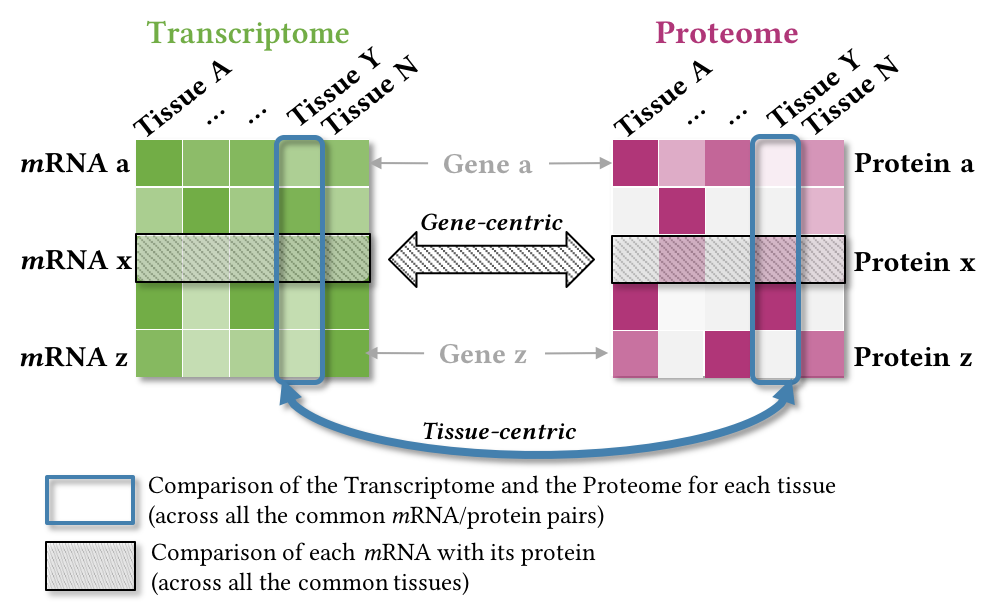
\includegraphics[scale=0.85]{integration/VisualExplaination-Lin.png}\centering
    %\vspace{-3mm}
    \caption[Summary of the expression comparison approaches between
    the transcriptome and proteome]{\label{fig:visualexp}\textbf{Approaches
    summary of the expression comparison between the transcriptome and proteome.}
    \emph{Tissue-centric} analyses focus on
    how the transcriptome and proteome relate to each other within the same tissue.
    \emph{Gene-centric} analyses study for each gene how its \mRNA\ expression
    levels across all (or a subset of) the tissues may relate to
    the quantified expression levels of its corresponding protein.
    }
\end{figure}

\Cref{fig:visualexp} summarises the two analytical approaches I use
to compare transcriptomic and proteomic data.
The \emph{tissue-centric} approach compares for each tissue
the global expression of its transcriptomic landscape to its proteomic one.
In contrast,
the \emph{gene-centric} approach compares for each gene
its expression levels in \mRNA\ and protein across all the tissues.
\afterpage{\clearpage\sectionmark{Fair correlations between independent proteomics and transcriptomics}}

Confusion can arise
when integrating proteomics and transcriptomics.
Hence, it is essential
to clearly define the taken approach~\mycite{Liu2016-re}.\mybr\
\vspace{-2mm}

\section{Fair correlations between independently sourced proteomics~%
and~transcriptomics~of~human~tissues~}\label{subsec:IntegrationGoodCorrProtTrans}
\sectionmark{Fair correlations between independent proteomics and transcriptomics}
\vspace{-2mm}

For the first tissue-centric analysis,
I assess for each tissue the relationship between
the expression of its proteome and transcriptome
through the correlation of the protein expression values
with their corresponding \mRNA\ ones.\mybr\

After scaling with $\log_2(x+1)$,
I compare proteomic and transcriptomic \treps\
from identical and random tissue pairs,
which are similar and roughly correspond to Gaussian distributions
as illustrated by \Cref{fig:distribTrans,fig:pandeyDistribQ1Q2}.

\Cref{fig:TestSig} presents the correlation distribution range
of transcriptomic and proteomic \treps\ from identical and random pairs of tissues
both with Spearman and Pearson correlation methods
(see \Cref{sec:CorrMore}).

Although transcriptomics and proteomics have independent sources,
the Spearman correlation of the same tissues \treps\ are equivalent to
correlations in cell studies~\mycite{Lundberg2010-gk,schwanhausserglobal:2011}
where a same sample provides \mRNAs\ and proteins.
Regardless of the protein quantification method
(Top3~\mycite{Silva-Top3} or \PPKM{} ---~\vref{eq:PPKM}),
the median Spearman correlation coefficients are above $0.5$
for matched proteomic and transcriptomic \treps\
(also referred to as \emph{same-tissue pairs}).
The unscaled data presents identical outcomes
(see \Cref{tab:pvalueCorrSP} and \Cref{fig:TestSigUnlog}).\mybr\

The Pearson correlation is closer to the literature
for our new \PPKM\ quantification
than for the Top3 quantification.
The \PPKM\ Pearson correlation averages
above $0.5$ $[$min:~$0.38$~(\Oesophagus)\;; max:~$0.61$~(\Liver)$]$
(and is within $[$min:~$0.45$~(\Oesophagus)\;; max:~$0.67$~(\Liver)$]$
for the untransformed data).\mybr\

\begin{figure}[!htbp]
    \includegraphics[scale=0.8]{integration/DFtestlog2.pdf}\centering
    \vspace{-4mm}
    \caption[Distribution of Pearson and Spearman correlation coefficients
    for same-tissue proteomic and transcriptomic pairs
    versus random tissue pairs]{\label{fig:TestSig}\textbf{Distribution of
    Pearson and Spearman correlation coefficients
    for same-tissue proteomic and transcriptomic pairs versus random tissue
    pairs ($\log_2$-scaled data).} Depending on the protein quantification method,
    there are two types of distribution ranges for the Pearson correlations.
    Top3 quantification method provides a lower correlation ($\text{mean} \approx 0.11$).
    The \PPKM\ method (\Cref{sec:NewQuantProt}) produces higher correlations
    ($\text{mean} \approx 0.5$).
    All the Spearman correlation ranges between same-tissue proteomic and
    transcriptomic \treps\ are quite similar,
    regardless of the method quantifying the proteins.
    The median of Spearman correlation is $0.52$.
    With the Top3 quantification (\ie\ pink countered boxes --- Top3 x HTSeq),
    two outliers are noticeable, and they are common to the three comparisons,
    Pandey x Uhlén (12 tissues and 15 tissues) and Pandey x GTEx (12 tissues):
    the lowest Spearman correlation is \Oesophagus\ ($\rho=0.39$)
    and the highest \liver\ ($\rho=0.62$).
    Both for the Pearson and Spearman correlations,
    even when the correlations are very low,
    same-tissue pairs always have higher correlations than
    different (random) tissues pairs
    (all p-values computed with Welch t-test <0.05 --- see \Cref{tab:pvalueCorrSP}).
    Thus, even the lowest same-tissue correlations are significative.
    The green boxplots, comparing the two transcriptomic datasets,
    are only represented for reference purposes.}
\end{figure}

\begin{figure}[!htbp]
    \includegraphics[scale=0.75]{integration/Kidney_scattplot_Q3_T15.pdf}\centering
    \caption[Scatterplot of protein (Pandey Lab data --- PPKM quantification)
    and mRNA (Uhlén \etal) expression for Kidney]
    {\label{fig:ScatKid}\textbf{Scatterplot of
    protein (Pandey Lab --- PPKM quantification) and mRNAs (Uhlén et al.)
    expression for Kidney.}
    Each point of this scatterplot represents a gene;
    it has the $\log_2$-transformed expression value
    of the corresponding \uhlen\ \etal\ \mRNA\ (\FPKM) on the x-axis and
    the $\log_2$-transformed expression value of
    the \pandey\ Lab protein (\PPKM) on the y-axis.
    Most of the \mRNA/protein pairs are distributed in an area
    that can be fitted by a linear function with a positive slope,
    which indicates a high correlation between \mRNAs\ and proteins expression
    levels.
    However, genes with lower expressed \mRNAs\ are more prone to dispersion,
    in particular, \mRNAs\ that are expressed below $1$ \FPKM\ (\ie\ below $0$ on
    the x-axis).
    On the other side, genes with the highest expressed \mRNAs\ may present
    a saturation effect (\Cref{subsec:simpleProt})
    in the quantification of the protein expression.
    The highest expressed protein is \protein{\gls{HBB}}
    (\ie\ Hemoglobin Subunit Beta), which is also found in
    the five highest expressed proteins in all the other tissues.
    Likely, its presence is due to remaining erythrocytes in the samples.
    On the outer parts of the scatterplot,
    there are the respective distribution densities of the proteins and the \mRNAs.
    Whilst the correlation calculation includes every pair of \mRNA\ and protein,
    the plot excludes any pair with a non expressed \mRNA\ or protein to optimise the visualisation.}
\end{figure}

As tissue proteomic samples can present high correlation
without being related in any manner
(see \Cref{ch:proteomics,fig:scat2DAdrenalPancreasKuster}),
a Welch t-test~\mycite{Welch1951-sj} allows
assessing the significance of the correlation for the same-tissue pairs
by comparison to random tissue pairs.
The one-sided \Welchttest\footnote{See \Cref{mini:ttest}}
allows rejecting the null hypothesis $H_0$
(the means of the correlation coefficients for same-tissues pairs
are identical or lower to random tissues pairs).
Irrespectively of the protein quantification or computational methods,
all the same-tissue pairs correlations are significant
(p-value $<5.10^{-5}$, except for Pearson correlation with Top3 quantification
where p-value $<0.05$ --- see \Cref{tab:pvalueCorrSP}).\mybr\

The previous correlation distribution
may imply a modest relationship between
these independent proteomics and transcriptomics,
but the same-tissue pairs scatterplots (\eg\ \Cref{fig:ScatKid})
show tighter links than first suggested.
Besides, these scatterplots share a coarse profile
despite the wide correlation ranges.\mybr\

\Cref{fig:ScatKid} illustrates the comparison of expression for \kidney\
between transcriptomics (\uhlen\ \etal) on the x-axis
and proteomics (\pandey\ Lab --- \PPKM) on the y-axis.
\Kidney's correlation coefficients stand in the middle of the range
regardless of the considered studies,
protein quantification or correlation methods involved in the comparison.

%To optimise the visualisation,
%I removed the pairs with a null member
%(either for the \mRNA\ or protein)
%while I keep them for the correlation calculation.


A linear function with a positive slope (not drawn) can fit the bulk of the points.
Indeed, the expression of most \mRNAs\ and proteins in a tissue are highly associated.
However, there is a high dispersion for the lowest ($<1$ \FPKM)
and many of the highest measured \mRNAs{}.

Besides the mismatching sampling sources,
other possible explanations for the dispersion are
technical limitations (such as protein saturation effect, see \Cref{subsec:simpleProt}),
translational noise (see \Cref{subsubsec:exprTrans})
or a consequent half-life difference between the \mRNA\ and its protein.

Although the number of genes concerned by the dispersion is rather limited,
they are enough to impair the Pearson and Spearman correlation coefficients.\mybr\

Systematic exclusion of the dispersal-prone genes
(either the proteins with lowly expressed \mRNAs\
or the highly expressed \mRNAs\ with a more limited protein expression)
is impractical and arguable
as they are inconsistent from one tissue to another.\label{memo:dispersedGenes}
Case-by-case treatment will be necessary.

Removing the lowly expressed \mRNAs\ ($<1$ \FPKM) only marginally changes
the correlation coefficients,
\eg\ for \kidney,
when considering the \PPKM\ quantification for the proteins,
the Pearson correlation
increases from $0.56$ to $0.58$,
while the Spearman correlation is relatively unchanged
($0.51$ instead of $0.52$).
The changes are relatively similar
when considering the more conservative Top3 protein quantification.
The Pearson correlation $r=0.18$ increases to $0.21$.
The Spearman correlation remains unchanged ($\rho=0.52$).

Regardless of the protein quantification method or
the transcriptomic study, %(either \uhlen\ \etal\ or \gtex\ study),
the results are essentially similar.
Thus, I mostly present thereafter the results of the most extensive set
(both in terms of tissues and genes),
\ie\ the fifteen-tissue set between \uhlen\ \etal\ and \pandey\ Lab data
(quantified with the \PPKM\ method).\mybr\

\vspace{-1mm}
The other combinations
(provided in \Cref{ch:SupplIntegration} or electronic format)
may diverge for individual genes through the various combinations,
but the general trends are identical.
\vspace{-1mm}

I focus on Pearson correlation over Spearman correlation\label{seg:pearOverSpear}
in the following parts
since the results for the \PPKM\ quantification are globally similar for both.
Additionally, Pearson correlations are easier to interpret
and more readily modelled upon for predictive purposes
(see \Cref{subsec:PearsonVsSpearman}).\mybr\
\vspace{-1.5mm}

\subsection{Mixed biological signal between the proteome and transcriptome
across the tissues}
\vspace{-8mm}
\begin{figure}[!hb]
    \includegraphics[scale=0.8]{integration/orderedHeatmapQ3Pearson.pdf}\centering
    \vspace{-3.5mm}
    \caption[Heatmap based on the Pearson correlation between protein and mRNAs
    expression (alphabetically ordered tissue)]{\label{fig:orderedHeatmapPearson}%
    \textbf{Heatmap based on the Pearson correlation between protein and mRNAs
    expression (alphabetically ordered tissue)}}
\end{figure}

%%%%%%%%%%%%%%%%%%%
%%%HERE%%%%%%%%%%%%%
As shown in \Cref{fig:orderedHeatmapPearson},
many proteomic \treps\ correlate the highest with
their corresponding transcriptomic \trep\
(\eg\ \liver, \testis, \ovary, \pancreas)
but other preferentially correlate with other tissues first
(\eg\ \bladder, \Oesophagus, \gallbladder).
Besides, depending on the chosen correlation methods,
a few tissues (\eg\ \heart) can have
their proteome and transcriptome correlate preferentially or not.\\
\vspace{-\baselineskip}

In order to identify possible factors
that influence the association strength
between the proteome and transcriptome,
I explore several avenues in the following sections.

I first study the effect of tissue composition (in proteins and \mRNAs)
on the correlations.
I begin with the assessment of the impact of the proteins and \mRNAs\
that are found in one tissue only,
before looking into the tissue-specific (\gls{TS}) proteins and \mRNAs{}.

Then, in a more quantitative approach,
I examine more closely how the \mRNA\ expression profiles relate
to their respective protein ones.

\subsection{Influence of the expression breadth on the tissue %
\texorpdfstring{\MakeLowercase{m}RNAs/proteins}{mRNAs/proteins} correlation}

Scatterplots of protein expression from different tissue pairs present
similar global profiles and correlation range to same tissue pairs
(see \Cref{ch:proteomics} and \Cref{fig:scat2DAdrenalPandeyPancreasKuster}).
In this context,
genes (expressed both as a protein and \mRNA)
uniquely found in one tissue can have a significant impact on the correlation.
Thus, their proportion per tissue may explain
the mitigated correlation results.%\\
%\vspace{-\baselineskip}

The expression breadth, presented in \Cref{fig:expressionBreadth},
allows visualising the number of tissues
where each gene (\mRNA\ or protein) is expressed.
\Cref{fig:protBreadth} shows that
the distribution of the protein expression breadth is bimodal.
Either due to technical limitations or biological reasons,
proteins detected in a sole tissue form
the most numerous class and represent 20 \% of the overall number.
Proteins expressed in all tissues are the second most numerous class (about $~$ 16 \%);
the third class (12 \%) comprises the proteins expressed in two tissues.

On the other hand,
almost all \mRNAs\ are expressed in every tissue (\Cref{fig:mRNAbreadth0}).
One hypothesis is that tissues express a protein only
if its corresponding \mRNA\ exceeds a sufficient threshold.
Thus, I also studied the effect of
two additional minimum expression thresholds for the \mRNAs\
on the expression breadth.\mybr\

The two new expression breadth profiles are more alike
to the proteomic one.
As shown in \Cref{fig:mRNAbreadth1},
the number of transcripts only found in one tissue increases
at the widespread $1$ \FPKM\ threshold,
which roughly equates to one \gls{RNA} in the cell~\mycite{Mortazavi2008,Hebenstreit:2011}.

The expression breadth profile of the \mRNAs\ expressed at or above $5$ \FPKM\
present a similar bimodal distribution (\Cref{fig:mRNAbreadth5}) to the protein one.
While arbitrary, $5$ \FPKM\ is a threshold commonly found
in the literature~\mycite{Uhlen2015,oneDominant,Chen2018-ln}.\\
\vspace{-\baselineskip}

\begin{figure}[!htb]
    \begin{subfigure}[h]{0.53\textwidth}
    \captionsetup{margin=0.6cm,justification=centering}
        \centering \includegraphics[width=\textwidth]{integration/breadthProtQ3--15.pdf}
        \caption{Protein~expression~breadth (\PPKM~quantification)}\label{fig:protBreadth}
    \end{subfigure}
    \begin{subfigure}[h]{0.53\textwidth}
    \captionsetup{margin=0.6cm,justification=centering}
        \centering \includegraphics[width=\textwidth]{integration/breadthmRNAQ3--15.pdf}
        \caption{mRNA~expression~breadth\\(> 0 \FPKM)}\label{fig:mRNAbreadth0}
    \end{subfigure}
    \vspace{2.5mm}

    \begin{subfigure}[b]{0.53\textwidth}
    \captionsetup{margin=0.6cm,justification=centering}
        \centering \includegraphics[width=\textwidth]{integration/breadthmRNAQ3--1501.pdf}
        \caption{mRNA~expression~breadth\\(≥1 \FPKM)}\label{fig:mRNAbreadth1}
    \end{subfigure}
    \begin{subfigure}[b]{0.53\textwidth}
    \captionsetup{margin=0.6cm,justification=centering}
        \centering \includegraphics[width=\textwidth]{integration/breadthmRNAQ3--1505.pdf}
        \caption{mRNA~expression~breadth\\(≥5 \FPKM)}\label{fig:mRNAbreadth5}
    \end{subfigure}
    \vspace{-5mm}
    \caption[Expression breadth of the proteins and mRNAs]{\label{fig:expressionBreadth}%
    \textbf{Expression breadth of the proteins and mRNAs.}
    Proteins have a bimodal breadth of expression.
    Many proteins are detected in one tissue only or all.
    Almost every \mRNA\ is detected in every tissue.
    Their breadth becomes bimodal when their expression threshold
    is increased to $5$ \FPKM{}.
    Note that the genes with null expression breadth are removed from the plots
    to ease the general visualisation.
    }
\end{figure}

\Cref{fig:UniqueFeatureQ3T15} shows the proteins and \mRNAs\
for which the expression breadth equates to $1$ in \Cref{fig:expressionBreadth}.
Instead of displaying the finite counts,
it displays the ratio across tissues,
\ie\ the number of unique feature (proteins or \mRNAs)
for each tissue divided by the total amount of them across all tissues.
The tissues are ordered in increasing order of their ratio in unique features.

\begin{figure}[!htb]
    \includegraphics[scale=0.78]{integration/uniqueFeatureQ3T15a.pdf}\centering
    \vspace{-3mm}
    \caption[Ratio across tissues of unique proteins and mRNAs]{\label{fig:UniqueFeatureQ3T15}
    \textbf{Ratio across tissues of unique proteins and mRNAs.}
    }
\end{figure}

Although their number (hence their proportion) varies from one tissue to another,
all fifteen tissues have proteins
that are specifically detected in each tissue solely
as shown in the top plot in \Cref{fig:UniqueFeatureQ3T15}.
In contrast, unique \mRNAs\ are detected in a more limited number of tissues
(see the three bottom plots of \Cref{fig:UniqueFeatureQ3T15}).
Besides, the unique proteins are more evenly distributed
between the fifteen tissues than the unique \mRNAs.

Except for \Testis\ and \Liver,
which are consistently expressing the highest number of unique features,
the other tissues lack to present any common pattern
between the available proteomic and transcriptomic data.

\Liver\ is the most correlated tissue (\Cref{fig:orderedHeatmapPearson})
and comprises the second-highest number of unique features.
\Testis\ is the third-best correlated tissue
despite having the highest ratio of unique proteins and \mRNAs\
(regardless of the threshold $0$ to $1$ \FPKM).
The other tissues lack to show any relationship
between their composition in unique features
and the correlation of their transcriptome and proteome.

Put together, these results suggest that
the tissues correlation levels are unrelated
to their amount of unique proteins and \mRNAs{}.
The lack of relation between the proteomic and transcriptomic observations
is confirmed by a more refined analysis of the expression breadth.

\begin{figure}[!htpb]
    \includegraphics[scale=0.75]{integration/coloredSharedbreadthProtQ3--15.pdf}\centering
    \vspace{-4mm}
    \caption[Comparison of the proteins expression breadth to their
    corresponding mRNA ones]{\label{fig:SharedBreadthProtQ3}%
    \textbf{Comparison of the proteins expression breadth
    to their corresponding mRNA ones.}
    This figure, where the protein expression breadth is coloured
    according to its comparison with the \mRNA\ one,
    is based on \Cref{fig:protBreadth,fig:mRNAbreadth5}.
    About one-fifth of the proteins that are detected in one tissue
    have their corresponding \mRNA\ (expressed at or above $5$ \FPKM{})
    presenting an \emph{identical} expression breadth.
    The number of proteins classified as \emph{Identical} decreases significantly
    for the other possible breadths
    except when all the tissues (\ie\ fifteen) are considered
    (then accounting for one-third of the proteins).
    Proteins with a breath of expression close to their \mRNAs{}' (± $2$)
    are identified as \emph{Similar}.
    If the protein and the \mRNA\ are both detected within four to nine tissues,
    they are described as \emph{Mixed}.
    If the \mRNA\ has been detected at or above $5$ \FPKM\
    but with another breadth than \emph{Identical} or \emph{Similar},
    it is then referred to as \emph{Different}.
    Finally, while many proteins are detected in one tissue (or even more),
    their corresponding \mRNAs\ are not at $5$ \FPKM\
    (\emph{Expression < $5$ \FPKM} category).
    }
\end{figure}

\Cref{fig:SharedBreadthProtQ3} shows that the expression breadth
of \mRNAs\ (expressed ≥ $5$ \FPKM\ or even smaller threshold) concurs
in very few cases to their corresponding protein one.
Thus, the \mRNAs\ expression breadth is
an ineffective predictor for the detection of a protein,
including extreme cases where the protein is unique to one tissue
or expressed in all fifteen of them.


All the expression breadth analyses of the transcriptome rely on expression levels.
However, \Cref{ch:Transcriptomics} underlines that
high expression levels of \mRNAs\ are unrelated to interstudy tissue correlation
while tissue-specific (\gls{TS}) \mRNAs\ present a rather strong connection with it.
For this reason, the following analysis examines
the relationship between \gls{TS} \mRNAs\ and \gls{TS} proteins.


\subsection{Tissue-specific \texorpdfstring{\MakeLowercase{m}RNAs}{mRNAs} %
have significant overlap with tissue-specific proteins}\label{sec:TSprotMrna}

Unlike \mRNAs,
many proteins are only expressed in one unique tissue.
These are the ones I refer to as \gls{TS} proteins in the remainder of this thesis.\mybr\

To enable the comparison of these \gls{TS} proteins with possible transcript counterparts,
I first order the \mRNAs\ in each tissue by specificity
with the method presented in \Cref{subsub:TisSpeGeneMethodPerso}
(\nameref{subsub:TisSpeGeneMethodPerso}).
Then, as detailed in \Cref{fig:RankSpe},
I examine for each tissue the overlap between its $n$ \gls{TS} proteins
with its $n$ \mRNAs\ with the highest tissue-specific ranks.
\Cref{fig:ExJacquard} illustrates the \heart\ example.
%\vspace{-\baselineskip}

\begin{figure}[!htb]
    \includegraphics[scale=0.59]{integration/TissueSpeDeter.pdf}\centering
    \vspace{-3mm}
    \caption[Determination process of the specific mRNAs]{%
    \label{fig:RankSpe}\textbf{Overview of the comparison of the TS proteins
    and TS mRNAs.}
    \gls{TS} proteins are the $n$ proteins only expressed in one tissue.
    Once the \mRNAs\ have been sorted
    by decreasing order of their relative specificity to a given tissue,
    the first $n$ \mRNAs\ identities are compared
    to the ones of the $n$ \gls{TS} proteins present in the same tissue.
    Jaccard's similarity coefficients and their significance (p-values)
    have been computed to allow
    a global assessment of the proteome and transcriptome relationship
    across all the tissues simultaneously.
    }
\end{figure}

\begin{figure}[!htbp]
\includegraphics[scale=0.63]{integration/overlapRatioPUQ15Q3Heart2.pdf}\centering
\vspace{-3mm}
    \caption[Example of overlap of TS proteins and TS mRNAs for Heart]{%
    \label{fig:ExJacquard}\textbf{Example of overlap of \gls{TS} proteins
    and \gls{TS} \mRNAs.}}
\end{figure}


Each tissue has a different number of \gls{TS} proteins.
I thus refine this analysis
by computing Jaccard similarity coefficients
(or Jaccard indexes)~\mycite{Jaccard1901-ei,Lin2008-fc}
(see \Cref{eq:Jaccard}).
The Jaccard indexes allow assessing
the relationship between \gls{TS} proteins and \mRNAs\
across all the tissues at the same time
and ease the result interpretation in contrast to the raw overlap numbers.
To measure their significance,
I use the hypergeometric test (see \Cref{sec:hypergeometricTest}).

\begin{minipage}{\textwidth}
    The Jaccard indexes for the generic case showed in \Cref{fig:RankSpe}
    is computed as follow:
\begin{equation}
    \tag{Jaccard similarity coefficient}\label{eq:Jaccard}
    \begin{split}
        J(x_{1},x_{2}) & = \frac{\left | x_{1}\cap  x_{2}\right |}%
                                {\left | x_{1}\cup  x_{2}\right |}\\
                       & = \frac{\left | x_{1}\cap  x_{2}\right |}%
                                {\left | x_{1} \right | + \left | x_{2} \right |%
                                - \left | x_{1}\cap  x_{2}\right |}\\
                                & = \frac{y}{2n-y} \text{\small{~(specifically
                                for~\Cref{fig:RankSpe})}}\\
    \end{split}
    \raisetag{6cm}
\end{equation}
\end{minipage}


\begin{figure}[!htb]
  %  \vspace{-5mm}
    \includegraphics[scale=1]{integration/overlapRatioPUQ15Q3.pdf}\centering
    \vspace{-2mm}
\caption[Heatmap of Jaccard indexes across 15 tissues]{%
\label{fig:JaccardIndexes}\label{fig:RatioJac}\textbf{Heatmap of Jaccard indexes
across the common fifteen tissues between Uhlén et al.\ and Pandey Lab data.}
For each tissue, the \gls{TS} proteins are the proteins
(quantified with \PPKM\ method) that are expressed only in that tissue.
The \gls{TS} \mRNAs\ are the \mRNAs\ with the highest specific coefficients
in that tissue.}
\vspace{-4mm}
\end{figure}

The Jaccard indexes for all pairs of the fifteen shared tissues
between the \pandey\ Lab (\PPKM\ quantification) and \uhlen\ \etal\
are summarised in \Cref{fig:JaccardIndexes},
while~\Cref{fig:JaccardPvalues} displays
their respective p-values (hypergeometric test).\\
\vspace{-\baselineskip}


As the number of \gls{TS} \mRNAs\ to compare is arbitrary,
I have rerun these analyses with $2*n$ \gls{TS} \mRNAs\ for $n$ \gls{TS} proteins.
While the raw numbers of overlapping features across the tissues increase,
the Jaccard indexes remain within the same ranges.

Regardless of the tissues, the datasets, quantification method of the proteins
or the chosen method to select the \mRNAs\
(either expression fold change or Hampel's method),
there is always some overlap between
the \gls{TS} proteins and the \gls{TS} \mRNAs\ candidates.
Except for (\tissue{Urinary}) \bladder\ (which has the smallest Jaccard index),
these overlaps are statistically significant
for all the commonly considered thresholds.

\vspace{-2mm}
Many of the highest correlated tissues have also the highest Jaccard indexes.
However, many inconstancies persist.
Thus, even though there are significant correspondences,
\gls{TS} proteins and \mRNAs\ are insufficient to explain
the correlation level between the proteome and transcriptome of each tissue.
\vspace{-\baselineskip}

\begin{figure}[!htb]
%\vspace{-2mm}
    \includegraphics[scale=1]{integration/overlapRatioPvalPUQ15Q3.pdf}\centering
    \vspace{1mm}
    \caption[p-values associated with the Jaccard indexes]{\label{fig:JaccardPvalues}\label{fig:pJacquard}%
    \textbf{p-value associated with the Jaccard indexes} of \Cref{fig:JaccardIndexes}.
    These p-values have been computed with the hypergeometric test.}
    \vspace{-3mm}
\end{figure}

The former direct approaches
(based on the gene expression breadth across tissues and their tissue-specificity)
lack to show a prominent (if any) contribution to the correlation levels
between the proteome and transcriptome.
These are most likely resulting
from a slew of subtle similarities
based on identical differential expression
within many clusters of the proteins and \mRNAs{}.%;
%while studying individually paired \mRNA/protein couples
%may not give any indications,
%smaller groups can present distinctive signals.
%cf. Pointillism mouvement.

As a direct and consistent hierarchical clustering
based on unique features is unreachable,
I have extended the analysis to examine whether or not an indirect method
may be more appropriate.
For this new approach,
I build hierarchical cluster trees that try to translate
the expression \enquote{closeness} of the tissues
(namely their differentiation distance).
Then, I compare the proteins' and transcripts' trees.\\
\vspace{-\baselineskip}

\subsection{Proteins and mRNAs tissue trees present partial concordant results\\}
\vspace{-12mm}

As presented in \Cref{subsec:clusteringPres},
a hierarchical clustering analysis requires a linkage method
and a distance measurement between each element that is included in the analysis.
For the linkage method, I use Ward's method~\mycite{Ward1963}
as in the previous analyses.

The distance must reflect the difference in composition of gene populations
that the tissues express.
To this end,
I only consider the proteins and \mRNAs\
that are expressed in two tissues strictly.
For each pair of tissues,
I count how many proteins or \mRNAs\ they share.
Then, I use the inverse of this number as a distance measure
since the larger the number of shared features,
the closer the tissues are.

\Cref{fig:separateTree} shows the hierarchical clustering for
\pandey\ Lab (\PPKM\ quantification)
and \uhlen\ \etal\ (≥ $5$ \FPKM)  studies,
while the number of shared features for \pandey\ Lab and \uhlen\ \etal\ data
are respectively showed in \Cref{fig:heatmapPandeyTissuePairs,fig:heatmapUhlenTissuePairs05}.

Both \pandey\ Lab and \uhlen\ \etal\ data present
the same three pairs of tissues more closely related:
\Testis\ and \Ovary, \Rectum\ and \hColon\ and \Liver\ and \Kidney.
\Cref{fig:consensus2D15TQ3} shows the consensus tree,
which is simpler to read.\\
\vspace{-\baselineskip}

Comparing more than two hierarchical trees is cumbersome manually;
thus, methods exist to create consensus trees~\mycite{Felsenstein2004-dv}.
One of the possible implementations is included in
the \textbf{\textsf{R}} package \softCi{ape \normalfont{(v5.2)}}{Paradis2019-ue}.
The methods can be strict or create a consensus based on the majority.
Since there is a maximum of three trees (one for each dataset)
to compare at a time,
all the consensus trees within this thesis are strict.

\Cref{fig:consensusTree05} relies on the set of twelve shared tissues between
\pandey\ Lab data (quantified by the \PPKM\ method)
and the two transcriptomic datasets (≥ $5$ \FPKM): \uhlen\ \etal\ and \gtex\ data.
Compared to \Cref{fig:consensus2D15TQ3},
only two tissue-sets are consistently found
as more closely related: \Testis\ and \Ovary, and \Liver\ and \Kidney.
Note that the results are identical
when I include the \pandey\ Lab data quantified by the Top3 method.


\begin{figure}[!htpb]
    \begin{subfigure}[b]{0.53\textwidth}
        \captionsetup{margin=0.6cm,justification=centering}
        \centering \includegraphics[width=\textwidth]{integration/TissuePairsQ3T15Pandey.pdf}
        \caption{Pandey Lab tissues\\(PPKM quantification)}\label{fig:treePandeyQ3T15}
    \end{subfigure}%
    \begin{subfigure}[b]{0.53\textwidth}
        \captionsetup{margin=0.6cm,justification=centering}
        \centering \includegraphics[width=\textwidth]{integration/TissuePairsQ3T15UhlenCut5.pdf}
        \caption{Uhlén et al.\ tissues\\(≥5 FPKM)}\label{fig:treeUhlenQ3T15cuth5}
    \end{subfigure}
    \vspace{-5mm}
    \caption[Tissues hierachical clustering for Pandey Lab and Uhlén \etal\ data]{\label{fig:separateTree}%
    \textbf{Hierarchical clustering for the fifteen tissues of
    Pandey Lab and Uhlén et al.\ studies.}
    }
\end{figure}

\begin{figure}[!htpb]
    \begin{subfigure}[b]{0.53\textwidth}
        \captionsetup{margin=0.6cm}
        \centering \includegraphics[width=\textwidth]{integration/TissuePairsQ3T15.pdf}
        \caption{Consensus tree of the fifteen common tissues between Pandey Lab
        and Uhlén et al. (≥ $5$ FPKM) data}\label{fig:consensus2D15TQ3}
    \end{subfigure}%
    \begin{subfigure}[b]{0.53\textwidth}
        \captionsetup{margin=0.6cm}
        \centering \includegraphics[width=\textwidth]{integration/TissuePairsQ3T123DFconsensus05.pdf}
        \caption{Consensus tree of the twelve common tissues
        between Pandey Lab data and
        Uhlén et al.\ and GTEx data (≥ $5$ FPKM)}\label{fig:consensusTree05}
    \end{subfigure}
    \vspace{-5mm}
    \caption[Tissues hierachical clustering for Pandey Lab and Uhlén \etal\ data]{\label{fig:consensusTrees}%
    \textbf{Consensus of the hierarchical clustering of the tissues across the different studies.}
    }
\end{figure}

When the consideration threshold of the \mRNAs\ is lowered to $1$ \FPKM,
\Liver\ and \Kidney\ are consistently observed as closely related
for every analysis based on the \PPKM\ method and
for the comparison of
the \pandey\ Lab quantified by Top3 with \uhlen\ \etal\ data.
Other tissue pairs are emerging as more related for a few comparisons:
\Rectum\ and \hColon\ for \pandey\ Lab and \uhlen\ \etal\ data,
with the addition of \Pancreas\ and \Gall\
when \pandey\ Lab is quantified by the \PPKM\ method.

At $0$ \FPKM, regardless of the quantification methods or included datasets,
no tissue structure is highlighted by the clustering.

Although these results are too mitigated, and
they lack to explain the correlation levels,
even indirect analyses based on the proteins and \mRNAs\ breadth expression
have some degree of similarity in their results.

Further more in-depth (direct or indirect)  analyses
may clarify the relationship between the proteome and transcriptome.
For example, equivalent correlation levels between specific gene groups
(gene co-expression correlation) may be highlighted
for each tissue at both biological layers.
However, this kind of analyses requiring a case-by-case approach
would greatly benefit from
well-established and proven \mRNA\ and protein expression baselines
for each tissue.


\section{Wide~correlation~range~for~protein/mRNA~pairs}
As previously reported, %(on p.~\pageref{memo:dispersedGenes}),
\mRNA/protein pairs can present
a tight relationship in one tissue
while being seemingly unrelated in another.
The first gene-centric analysis explores for each gene
the relationship between the expression levels of its \mRNAs\ and proteins
across all the available tissues.
This analysis helps to determine
whether any intrinsic trend structures the gene expression or
or if it is only subjected to their environment nature.

\begin{figure}[!htb]
    \includegraphics[scale=0.9]{integration/PearsonLog2correlationRankedGenes3-15-seed-1254.pdf}\centering
    \vspace{-2mm}
    \caption[Pearson correlation coefficients of \mRNA/protein pairs expression
    across the common tissues in descending order]
    {\label{fig:GeneProtCor}\textbf{Pearson correlation coefficients of \mRNA/protein
    pairs expression across the common tissues in descending order.}
    For each couple of an \mRNA\ and its corresponding protein,
    I have computed their Pearson correlation (in pink)
    across the fifteen common tissue
    between \pandey\ Lab (\PPKM) and \uhlen\ \etal\ data
    and then ordered them in decreasing order.
    The x-axis shows the rank of each pair
    and the y-axis its correlation coefficient
    (computed with $\log_2(\text{level}+1)$).
    The grey line represents one of the 10,000 randomisations
    (by pair composition permutation).
    This simulation iteration (and all the others) confirms
    that the observed correlation coefficients are
    significantly higher than expected.
    The green line serves as a possible \emph{ideal} case:
    it represents the Pearson correlation of \mRNAs\ pairs
    between \uhlen\ \etal\ and \gtex\ data
    (across their shared twenty-three tissues).
    }
    \vspace{-1em}
\end{figure}

Note that \Cref{app:geneCentric} regroups more complementary results
(including the \gtex\ data and those based on the Spearman correlation).
Since they all share overall identical trends,
I only present herein one set of results based on the Pearson correlation
(and for the same reasons mentioned previously in \Cref{seg:pearOverSpear}
(p.~\pageref{seg:pearOverSpear})).

\Cref{fig:GeneProtCor} displays the Pearson correlation
of the matching pairs of \mRNAs\ from \uhlen\ \etal\
and the proteins from \pandey\ Lab (quantified with the \PPKM\ method)
across their fifteen common tissues.
The observed levels of correlation (in pink)  are greater
than the expected levels (in grey) computed by random permutation.

I also compare the Pearson correlation of the matching \mRNAs/protein pairs
with the ones (in green) of the \mRNAs{}/\mRNAs\ pairs
from \uhlen\ \etal\ and \gtex\ data
to provide more context.
About one-third of the genes present a debatable level of correlation
between the two transcriptomic studies
(4,371 \mRNAs\ present a Pearson correlation coefficient below $0.8$).
On the other hand,
most of the \mRNA/protein pairs have a coefficient lesser than $0.8$,
as only 775 present a coefficient greater than or equal to $0.8$.

The Pearson correlation ranges rather widely:
from $1$ (for 27 pairs)
to below $-0.5$ (for 105 pairs,
with $r=-0.83$ for the  most anticorrelated one).\mybr\

A closer look at both extremes (\Cref{fig:caseGene} --- p.~\pageref{fig:caseGene})
reveals several possible relationship profiles
between the expression of the \mRNAs\ and proteins.
The negatively correlated genes can present
overall anticorrelated or rather unrelated expression levels
of \mRNAs\ and proteins.
On the other end,
the highest correlated genes present
tightly related \mRNA\ and protein expression levels
or a tissue-specific (\gls{TS}) protein.

\begin{figure}[!htb]
    \begin{subfigure}[h]{0.5\textwidth}
        \captionsetup{oneside,margin={0.8cm,0cm},justification=centering}
        \centering \includegraphics[width=\textwidth]{integration/antiCorrelated.pdf}
        \caption{Anticorrelated}\label{fig:caseAnticor}
    \end{subfigure}~%
    \begin{subfigure}[h]{0.5\textwidth}
        \captionsetup{oneside,margin={0.8cm,0cm},justification=centering}
        \centering \includegraphics[width=\textwidth]{integration/antiModerateCorrelated.pdf}
        \caption{Uncorrelated}\label{fig:caseUncor}
    \end{subfigure}
    \vspace{2mm}

    \begin{subfigure}[h]{0.5\textwidth}
        \captionsetup{oneside,margin={0.8cm,0cm},justification=centering}
        \centering \includegraphics[width=\textwidth]{integration/fairlyCorrelated.pdf}
        \caption{Well correlated}\label{fig:caseFairlyCor}
    \end{subfigure}~%
    \begin{subfigure}[h]{0.5\textwidth}
        \captionsetup{oneside,margin={0.8cm,0cm},justification=centering}
        \centering \includegraphics[width=\textwidth]{integration/PerfectlyCorrelated.pdf}
        \caption{Perfect correlation}\label{fig:casePerfectlyCor}
    \end{subfigure}
    \caption[Different cases of correlation
    protein/mRNA]{\label{fig:caseGene}\textbf{Different cases of correlation
    protein/mRNA.} The high correlated ones are enriched in pairs that are
    Tissue-specific (TS) as \mRNA\ and protein.}
\end{figure}

\FloatBarrier\

\subsection{TS~protein~enrichment~for~the~most~correlated~pairs}
\vspace{-5mm}
In the next analysis, illustrated in \Cref{fig:Spe_Cor},
I estimate if the highly correlated \mRNA/protein pairs
are predominantly due to tissue specificity
by computing the proportion of \gls{TS} proteins
for each rank of correlation presented in \Cref{fig:GeneProtCor}.

\begin{figure}[!ht]
    \includegraphics[scale=0.88]{integration/TSratioBasedOnPearsoncorrelationRankedGenes3-15-seed-1279.pdf}\centering
    \vspace{-3mm}
    \caption[Course of the TS proteins ratio and the Pearson correlation
    of protein/mRNA pairs]{\label{fig:Spe_Cor}%
    \textbf{Course of the TS proteins ratio and the Pearson correlation
    of the protein/mRNA pairs across the fifteen tissues.}
    The two parts of the figure share the same x-axis
    that displays the Pearson correlation ranks (decreasing order) of each pair.
    The upper plot is based on \Cref{fig:GeneProtCor}
    and shows as its y-axis the Pearson correlation coefficient
    of the protein/\mRNA\ pairs.
    The lower plot shows on its y-axis
    the cumulative proportion of \gls{TS} proteins up to each rank
    (\ie\ the ratio of \gls{TS} proteins
    within the set delimited from the highest correlated pair
    to the currently considered one).
    The data of the three categories (and colours)
    are identical to \Cref{fig:GeneProtCor}.}
\end{figure}

\vspace{-1mm}
\Cref{fig:Spe_Cor} illustrates the relation between the \gls{TS} protein ratio
and the Pearson correlation of the protein/\mRNA\ pairs.
Overall, one-fourth of all the pairs have a \gls{TS} protein.

The most correlated protein/\mRNA\ pairs display
a clear-cut enrichment in \gls{TS} proteins.
On the other hand, the corresponding \mRNA/\mRNA\ pairs present a weak one,
and the most correlated randomised protein/\mRNA\ pairs
lack to show any enrichment.
Most of the pairs comprising a \gls{TS} protein have
a Pearson correlation above 0.5,
although they show a wide range of Pearson correlation,
from $r=1$ to $r= -0.77$ for \gene{ZNF770}.\\
\vspace{-\baselineskip}

As mentioned previously,
either artefacts or biology may explain the observed low correlated pairs.
It is rather difficult to point
which artefacts are specifically impacting each protein/\mRNA\ pair
as there are many and can occur in combination.
However, two major technical sources of artefacts,
which have been reported,
are dispersion for the lowly expressed \mRNAs\ and
saturation for the highly expressed proteins.
See \Cref{sec:transExplo,sec:exploreProtMS} (from p.~\pageref{sec:transExplo})
for more details.
\vspace{-2mm}

\begin{figure}[!htb]
    \includegraphics[scale=0.57]{integration/TissueCorInterp}\centering
    \vspace{-3mm}
    \caption[Possible mRNA/protein expression profiles
    due to biological reasons.]{\label{fig:CorImprovable}%
    \textbf{Possible mRNA/protein expression profiles due to biological reasons.}
    Genes with well-correlated transcriptomic and proteomic expression
    are found in the grey area delimited by the green line.
    The genes in the yellow area,
    \ie\ which present a high concentration of protein for a small \mRNA\ one,
    may have stable proteins and \mRNAs\ with short half-lives.
    The genes in the blue area,
    genes with a low concentration of proteins but a high concentration of \mRNAs\
    may have a highly regulated translation,
    a protein challenging to capture
    or a misfit between the annotation definition of their \mRNA\ and protein.
    }
\end{figure}


\Cref{fig:CorImprovable} shows possible profiles of correlation for
protein/\mRNA\ pairs.
While explanations are usually disregarded or unrequired for genes
with well-correlated protein and \mRNA\ expression
(the grey area delimited by the green line),
other, less correlated, genes may need more context.

Genes in the yellow area,
\ie\ that present a high concentration of protein for a low \mRNA\ one,
may be due to stable proteins with short half-lives \mRNAs{}.
On the other side,
genes with a low concentration of protein with a high \mRNA\ one
may be explained by a high level of regulations for their translation
or by proteins challenging to capture
(either because of unsuited protocols or annotation misfits).
Note that genes sharing the same profile as \gene{SSR3} (\Cref{fig:caseAnticor})
might indicate self-regulation processes.

At the time of writing,
the most accurate way to classify the protein/\mRNA\ pairs
is to visualise the expression of each pair across the different tissues
(and dataset combination).

Instead, in the next section, I favour a more general approach.
I study through downstream analyses (see \Cref{sec:enrichmentAnalysis})
several genes groups
to find possible biological factors that may differentiate them.

\subsection{Distinct functional enrichment profiles
for pairs with a TS protein,
and~for~the~best~correlated~and~most~anticorrelated~ones}

As a downstream analysis,
I perform an enrichment analysis,
namely a \glsdesc{goa} (\gls{goa} --- see \Cref{sec:goaGeneralities}).

This analysis uses gene ontologies that provide defined terms
covering the gene product (\ie\ \mRNA\ and protein) properties.
These terms are structured into categories.
It helps to assess whether a set of genes is associated with
a biological process (BP), a molecular function (MF) or a cellular component (CC).
The three ontologies are included
in the \gls{BiocR} package \softCi{org.Hs.eg.db}{orghsegdb}
for analysis in \WebFoCi{\textsf{R}}{https://cran.r-project.org/}{coreR}.

The enrichment computation requires
the comparison between the \gls{go} terms set associated
with each studied list of genes to a reference.
I consider three genes lists:
the three hundred best correlated and
the three hundred most anticorrelated protein/\mRNA\ pairs
and all the pairs (2,613) with a \gls{TS} protein.
As a reference, I use the 12, 921 matching protein/\mRNA\ pairs
between \pandey\ Lab (\gls{PPKM} quantification) and \uhlen\ \etal\ data.

The \gls{BiocR} package \softCi{clusterProfiler \normalfont{(v3.12)}}{clusterProfiler}
provides a function \textsf{enrichGO},
which implements the \gls{goa} as the over-representation test
described by~\citet{Boyle2004-dh}
and handles all the required statistical testing
and (Benjamini and Hochberg~\mycite{Benjamini1995-nf}) correction.

%\begin{landscape}
    \begin{sidewaysfigure}
        \includegraphics[scale=0.95]{integration/goea.pdf}\centering
        \vspace{-3mm}
        \caption[Enriched GO categories for the pairs with a TS proteins and for the
        three hundred best correlated and most anticorrelated
        ones]{\label{fig:goares}%
        \textbf{Enriched GO categories for the pairs with a TS protein
        and for the three hundred best correlated
        and most anticorrelated ones.}
        The shared y-axis of the two parts includes the enriched GO categories
        (for any of the three groups).
        The left part of the figure shows
        a heatmap where all the included protein/\mRNA\ pairs (\ie\ 3,213)
        are sorted by their Pearson correlation on the x-axis and
        that each association of a pair with a \gls{go} category is marked.
        The right part shows the results from the comparison
        of the BP \gls{goa} analysis with \soft{clusterProfiler},
        where the three groups are on the x-axis with their number of genes
        annotated in the considered ontology.
        For each dot, the size represents the ratio of pairs within each group
        contributing to each category enrichment,
        and the colour indicates their significance.
        }
    \end{sidewaysfigure}
%\end{landscape}


Although the lists of the best correlated pairs and
the ones with a \gls{TS} protein present distinctive enrichment profiles
through the three ontologies,
the most anticorrelated pairs list presents
an enrichment only for biological process (BP) terms.

\Cref{fig:goares} presents the results for
the comparison of the enrichment of the three considered gene lists
for the BP ontology.

The left side of the figure is a heatmap
that marks the pairs' associations to the \gls{go} categories on the y-axis.
It includes all protein/\mRNA\ pairs of the three studied gene lists.
They are sorted on the x-axis in decreasing order of their Pearson correlation.

These \gls{go} categories, shared between both sides of the figure,
combine the five most enriched categories
for each of the three lists (\gls{TS} proteins, best correlated
and most anticorrelated pairs).
The categories enrichment is provided by another \soft{clusterProfiler} function,
\textsf{compareCluster} (which internally invokes \textsf{enrichGO}),
which has also produced the right side plot.\\
\vspace{-\baselineskip}
%The numbers under each list label (x-axis) are the number of genes
%in that list for which \gls{go} terms exist in the considered ontology (here BP).
%The size of the dots gives the enrichment
%as it is the ratio of pairs associated with terms of the \gls{go} categories
%within each studied list.

Note that while a few genes are enriched for \gls{go} categories primarily
associated with the pairs with \gls{TS} protein and one of the two others lists
(as visible on the heatmap),
no cross-enrichment exists
(ensured by the \enquote{\textsf{includeAll=TRUE}} option).\\
\vspace{-\baselineskip}

Strikingly, the \gls{go} categories associated with each gene list create
coherent groups of similar biological processes.
The pairs with \gls{TS} proteins are enriched in terms for specific signalling,
either for its detection (\enquote{\textit{detection of chemical stimulus}},
\enquote{\textit{sensory perception of chemical stimulus}},
\enquote{\textit{sensory perception}}),
as answer to a signal (\enquote{\textit{G protein-coupled receptor signalling pathway}})
or as a regulation (\enquote{\textit{regulation of signalling receptor activity}}).

Concurrently, the best correlated pairs are associated with catabolic processes\footnote{%
Catabolic processes are an energy release source
and depend on molecules requiring to be break down~\mycite{molBiolCell}.},
and the most anticorrelated ones are related to
ribosomes and \glspl{ncRNA} regulation,
thus by extension to the translation.

All the individual enrichment \gls{go} analyses
along with the comparison of the enrichment for the CC and MF ontologies
are provided as supplementary material.

The \gls{go} terms enrichment analysis with the CC ontology shows
that the best correlated genes are the most enriched
for the following categories:
the \enquote{\textit{postsynaptic membrane}},
\enquote{\textit{apical plasma membrane}},
\enquote{\textit{apical part of cell}},
\enquote{\textit{cluster of actin-based cell projections}},
\enquote{\textit{brush border}}
and the \enquote{\textit{cornfield envelope}}.\mybr\

On the other hand, the pairs presenting a \gls{TS} protein
show a slight enrichment for
\enquote{\textit{ion channel complex}},
\enquote{\textit{transmembrane transporter complex}},
\enquote{\textit{transporter complex}},
and \enquote{\textit{cation channel complex}}.
While the enrichment of the best correlated genes relays on more genes,
the categories of this list are located more specifically in subsets of cells,
whereas the categories associated to the \gls{TS} proteins
are more ubiquitous and can concern every cell type.
The localisation of the best correlated pairs probably suffers
from their overall ubiquity,
and thus, it is probably an artefact.

The enrichment analysis with the MF ontology
for the best correlated pairs points to different activities:
oxidoreductase, cofactor and transmembrane transporter or signalling activities
(\enquote{\textit{anion transmembrane transporter activity}},
\enquote{\textit{oxidoreductase activity, acting on CH-OH group of donors}},
\enquote{\textit{oxidoreductase activity, acting on the CH-OH group of donors
NAD or NADP as acceptor}},
\enquote{\textit{cofactor binding}},
and \enquote{\textit{coenzyme binding}}).

The pairs with a \gls{TS} protein are also associated
transporter and signalling activities
(with the following fifth categories:
\enquote{\textit{transmembrane singling receptor activity}},
\enquote{\textit{signalling receptor activity}},
\enquote{\textit{molecular transducer activity}},
\enquote{\textit{channel activity}},
and \enquote{\textit{passive transmembrane transporter activity}}).

Put together, these results suggest that
when there is a high correlation or anticorrelation,
biological processes are more into play than the possible technical ones.

The anticorrelated pairs lack to present any enrichment
for a specific cell compartment or a molecular function.
Thus, it implies that
regardless of their localisation within the cell
or their chemical properties (which relate to their molecular function),
the bottom-up \ms\ studies manage to capture most of the proteins
with variable effectiveness.

Nevertheless, bottom-up \ms\ studies favour some proteins,
and missing proteins are a primary source of ambiguities~\mycite{Poverennaya2017-vm}.
Hence, comparing the relative expression levels of proteins within a tissue
may induce misinterpretations.
On the other hand, while it requires caution,
the relative expression levels of each protein across tissues
ought to provide biological insights.

Finally, running all the gene-centric analyses presented here
after removing the negatively and anticorrelated pairs of \uhlen\ et al.\ and
\gtex\ \mRNAs\ give substantially similar results.

\section{Discussion}

In this chapter,
building on the insights gained in previous chapters
(particularly \Cref{ch:Transcriptomics,ch:proteomics}),
I have restricted the integration study to
the three following independent sources:
\uhlen\ et al.~\mycite{Uhlen2015}
and \gtex~\mycite{GTExTranscript} data for the transcriptomics
and \pandey\ Lab data~\mycite{PandeyData} for the proteomics.
The three datasets share twelve tissues,
while the working sets based on \uhlen\ et al.\ and \pandey\ Lab data
include three more tissues.
According to the considered working set and protein quantification methods,
the various analyses encompass 6,357 to 12,921 \mRNA/protein pairs
(respectively
three datasets --- state-of-the-art protein quantification (see \Cref{ch:datasets})
and two datasets --- new quantification method presented in \Cref{ch:proteomics}).
I have used both tissue- and gene-centric approaches
for their comparison and integration.\mybr\

The tissue-centric analyses show that
even independently sourced proteomics and transcriptomics of similar tissues
present fair correlation coefficients,
\eg, for Spearman $\rho_{\text{(\Oesophagus)}}=0.39$
$≤$ $\rho_i$ $≤$ $\rho_{\text{(\liver)}}=0.62$.
This correlation range is consistent with the literature,
either published before this study or in the meanwhile (see examples further forward).

More rivetingly,
the new \PPKM\ quantification method for proteins,
presented in \Cref{ch:proteomics},
enables reaching the same \emph{Pearson correlation} range
($r_{\text{(\Oesophagus)}}=0.38$ $≤$ $r_i$  $≤$ $r_{\text{(\liver)}}=0.61$)
that is usually achieved by cell studies specifically designed
for the joint integration of \emph{same-sourced} proteomics and transcriptomics
(\eg, \citet{Marguerat2012-sn,schwanhausserglobal:2011,Schwanhausser2013-et,Li2014-ai}).
Spearman correlation is the literature standard.
However, I have based my following considerations and discussion
on the Pearson correlations
since they are more easily interpretable.

Either due to biological reasons or technical ones (\eg\ saturation effects%
\footnote{For example, \citet{TOP3isbetter} report that
\ms\ label-free absolute quantification proteomics underestimate
a large dynamic range of proteins.})
the proteome displays a more stable expression across
tissues~\mycite{Laurent2010-rg,KusterData,PandeyData,GTExTranscript}.
Among the one hundred highest expressed proteins,
70\% are ubiquitous in the forty-seven tissues examined by \citet{KusterData}.
\citet{PandeyData} have identified 2,350 genes encoding for proteins
that they found across all the human cells and tissues they studied.
They estimated that these \enquote{housekeeping proteins} are
highly abundant as they are accounting for approximately 75\% of total protein mass
(based on spectral counts).
Despite the tissue proteomic expression profiles closeness,
all the same-tissue paired transcriptomic/proteomic \treps\
are statistically significant, even the least correlated ones.

To better understand the mixed level of correlation across tissues,
I have considered several properties as possible driving factors.
I have compared the expression breadth of the \mRNAs\ and the proteins
before comparing together the most specific proteins and \mRNAs\ of each tissue.\mybr\

Even though \mRNAs\ and proteins expression breadth distributions share
the same overall shape,
the concordance is only partial between them
(\ie\ the expression breadth of an \mRNA\ and its corresponding protein).
While unable to correctly explain the different correlation levels of the tissues,
this analysis highlights noteworthy facts
--- including a few recently reported in the literature;
\testis\ displays the most unique and diverse expression
both at transcriptomic and proteomic levels
(see also \citet{Wang2019-ut,Zhang2015-yn});
\liver\ (the most correlated tissue) present the second-highest number
of \mRNAs\ and proteins with a unique expression breadth.
Besides, the expression breadth of an \mRNA\ is mostly unhelpful
to predict the expression breadth of its corresponding proteins directly.
Inversely, when the expression breadth of a protein is unique,
the expression breadth of its related \mRNA\ is also more likely to be unique
at the threshold of 1 or 5 \FPKM{}.

Nonetheless, \mRNAs{}' and proteins' expression breadths carry partly on
the biological signal.
From the proteins and \mRNAs\ solely expressed in two tissues,
I have built hierarchical trees,
and their consensus tree outlines
the \ovary{}/\testis{} and the \kidney{}/\liver{} clusters
at both proteomic and transcriptomic layers.\mybr\

As shown in \Cref{ch:Transcriptomics},
most tissue-specific (\gls{TS}) \mRNAs\ give better
interstudy tissue correlation
than the highest expressed ones.
The overlaps between the $n$ \gls{TS} proteins and
the $n$ most \gls{TS} \mRNAs\ of each tissue are non-empty,
and except for one tissue (\tissue{Urinary Bladder}),
statistically significant with an $\alpha$ level of $0.01$.
The tissues with the highest overlaps are
also the ones with the highest correlation
between their transcriptomics and proteomics.
Unfortunately, this analysis lacks to explain
the whole correlation range.\mybr\

The gene-centric analyses show on the other hand that
about $6\%$ of the \mRNAs/proteins are highly correlated ($r_i≥0.8$),
about $18\%$ of them are well correlated ($0.8 < r_i ≤ 0.5$),
about $75\%$ of them are poorly correlated ($0.5 < r_i ≤ -0.5$), and
less than $1\%$ of the pairs are anticorrelated ($-0.5 < r_i ≤ -0.83$).

A fourth of the \mRNA/protein pairs included in this study have a \gls{TS} protein.
They considerably enrich the set of most correlated pairs.
Although most of them have a Pearson correlation above $0.5$,
their correlation ranges rather widely ($1 ≤ r≤ -0.77$).

Finally, I have investigated with a \gls{go} enrichment analysis
whether the three groups of \mRNA/protein pairs
(the ones with a \gls{TS} protein, the best correlated pairs
and the most anticorrelated ones) are relating to
any biological or technical reasons.

While the most correlated pairs and the ones including a \gls{TS} protein
present an enrichment in biological process (BP),
molecular function (MF) and cellular component (CC) terms,
the anticorrelated pairs present an enrichment only in BP terms.
Overall, the pairs with a \gls{TS} protein are most likely involved
with specific signalling (its detection, transduction or answer)
and more concentrated in the transmembrane area.
The most correlated \mRNA/protein pairs seem highly associated
with catabolic processes,
while the most anticorrelated ones to regulation processes.

It is imperative to remember that the proteome and the transcriptome used
for these analyses are independently sourced and aggregated from several individuals.
Many genes displaying mitigated correlation in my analyses will most probably
present high correlation or anticorrelation in matched samples.
The most affected genes are the most sensitive ones
to inter-individual variation and batch effects.

On the other hand,
current high-throughput technologies
for proteomics and transcriptomics give a picture of gene expression
at a specific time
since it fluctuates through time.
Even though bulk \Rnaseq\ and \ms\ give an average expression
of all the cells in each tissue,
the latter may express differently through time or condition.
Possible examples include premenopausal \Ovary\ and \Uterus.
Besides, related pairs of ubiquitously expressed \mRNAs\ and proteins
highly correlated or anticorrelated require subtle different interpretations
than in studies designed primarily for integration purposes.
In the context of my analyses,
except a limited number of spurious ones,
the highly correlated (or anticorrelated) pairs have
the most robust expression across individuals, through time,
and are less subjected to technical noise.

Correlations are dependent on the quantification of identified molecules.
Hence, the \mRNA\ and protein respective stability of each pair has
a direct impact on their quantification.
Therefore on their correlation too.
\citet{Vogel2012-sq}'s review reports several papers
--- including \citet{schwanhausserglobal:2011} ---
that have observed higher expression stability for
\glspl{RNA} and proteins related to mammalian metabolism
while proteins involved in transcriptional regulation (and chromatin organisation)
tend to degrade rapidly.\mybr\

The relative stability may be the sole reason behind the observed correlations here.
Other biological or biochemical reasons may also be at play.

If we accept the premise that
identical regulation steps apply across all tissues
to each highly correlated or anticorrelated \mRNA/protein pairs,
the previous results suggest that
catabolic genes are less regulated than other genes,
and
regulation genes may involve negative self-regulating mechanisms.
Nevertheless, the latter group requires more caution
since anticorrelated genes are harder to interpret.\mybr\

The highest protein-per-mRNA ratios observed
for mammalian metabolic genes~\mycite{Vogel2010-ux} tends
to back the more limited regulation for the catabolic genes.

Furthermore, it seems that regardless of each individual's particulars
(\eg\ sex, alimentary diet, age, physical level),
many catabolic gene expression only varies according to the tissue.
As organs have different metabolic profiles~\mycite{Berg2002-vo},
further studies may identify specific catabolic signatures for each tissue.

Another possible follow-up study can investigate
the potential of these molecules' concentration in each tissue
as a regulating factor for catabolic genes.
If proven significant,
it can contribute to the plausibility of the hypothesis that
catabolic genes are less regulated
by peri-transcriptional and posttranslational mechanisms.

It also may worth exploring across the tissues
whether these catabolic genes share particular coexpression profiles
with genes involved with the active or passive transport of the molecules
to be degraded (\eg\ transmembrane channel proteins).

On the other hand,
besides the poor protein stability,
the anticorrelated pairs may also result from technical artefacts.
In addition to the saturation effect (see \Cref{subsec:simpleProt})
and the degenerate peptides (see \Cref{subsec:proteinInference}),
other discrepancies can exist.
Many quantification inconsistencies exist
between methods, platforms and studies~\mycite{Dapas2017-ui,Aebersold2018-jn}.
Additionally, the same method can yield different quantifications
with slight variations in a few factors.
A possible example of oft-neglected sources is the gene length.
While normalisation methods for \Rnaseq\ require the genes or transcripts length
(see \Cref{subsub:norm}),
I chose to perform all the analyses at gene level expression
(see p.~\pageref{minisec:quantNorm}).
In fact, there are for each gene various \mRNA\ isoforms~\mycite{MarPhD}
and proteoforms~\mycite{Aebersold2018-jn}
and currently many criticisms exist about
the algorithms' accuracy at isoform level~\mycite{tamaraRNA,ernestRNA,Dapas2017-ui}.\mybr\

To keep congruity with the gene length
employed by \WebFoCi{\egxa}{https://www.ebi.ac.uk/gxa/home}{EBIgxa},
I use the sum of the lengths of all its collapsed exons.
The metapipeline
\softFoCi{\irap}{https://nunofonseca.github.io/irap/}{Fonseca2014-si} provides
graciously these gene lengths computed in this manner.
Yet, most genes present one dominant transcript~\mycite{oneDominant}.
One possible method to improve the \mRNA/protein correlations
is to identify the most dominant transcript isoform of each gene
and use their length for the normalisation.
This method ought to be rather easy to implement,
either through a first data analysis
or with the help of resources like
\WebFoCi{APPRIS}{http://appris-tools.org/}{Rodriguez2018-fk}.

More generally,
besides improving current results,
(even partial) better identification of the \mRNAs\ and proteins isoforms
will most likely also unveil still undetected divergences
between \mRNA\ and protein expression.\mybr\

Another source of discrepancy is the annotation.
For example, \gene{STAU2} (Pearson $\r=-0.59$  --- Spearman $\rho=-0.65$)
appears to be known to have different annotations
in the proteomic and transcriptomic communities.

Among the studies published in the meantime of my thesis' works and redaction,
three are most notably pertinent to the comparison and integration analyses
I have outlined above.

A first published comparison~\mycite{SciRep2016} of the expression data of
\gtex\ \mycite{GTExTranscript} and the \pandey\ Lab~\mycite{PandeyData}
provides weaker results than the above presented ones.
The authors have based their complete study on data provided as-is
by the \gtex\ project and the \pandey\ Lab.
Hence, although the primary resources are useful
for other authors to praise the presence of a given gene in a particular tissue,
more extensive uses need more considerations
and probably some preliminary treatments.

\citet{Franks2017-bp} integrate a subset of the \uhlen\ data included
in this chapter analyses
as they have extracted their transcriptomic data as-is from \citet{Uhlen2014}
to integrate it with the data they have reprocessed
from \citet{PandeyData} and \citet{KusterData}.
The study's primary aim is
to quantify the post-transcriptional regulation of the genes
through their translational efficiency.
To this end, they compute for each gene a \emph{\gls{PTR}}.
\glspl{PTR} ease the assessment of the gene expression variability
across their set of tissues.
This study underlines the utmost caution required
when one considers the transcriptome as a possible proxy for the proteome.
Besides, it also reminds that data quality and reliability are primary caveats
for possible analyses.
However, \citet{Franks2017-bp} show that genes from a same set of \gls{go} terms
display similar \gls{rPTR} profile across tissues,
\ie\ they have higher and lower \gls{rPTR} in the same tissue sets.
This observation suggests a concerted functionally regulations.

The last study by~\citet{Wang2019-ut} is a follow-up of a series of previous ones.
All have been conducted on the same set of human tissues samples
collected by the Department of Pathology,
Uppsala University Hospital, Uppsala, Sweden,
as part of the sample collection governed by
the \WebFo{Uppsala Biobank}{https://www.uppsalabiobank.uu.se/en/}.
This study involves matched transcriptomic and proteomic data sourced
from the same samples.
The transcriptomic data is one of the datasets used in this chapter's analyses:
the \uhlen\ \etal\ data~\mycite{Uhlen2015},
which raw data can be downloaded from \gls{ArrayExpress}\footnote{%
\ArrayExpress{\href{https://www.ebi.ac.uk/arrayexpress/experiments/E-MTAB-2836/}{E-MTAB-2836}}
---\\ \Href{https://www.ebi.ac.uk/arrayexpress/experiments/E-MTAB-2836/}}.
The proteomic data has been referenced for the first time by~\citet{Wang2019-ut}
and can be retrieved in \gls{Pride}\footnote{%
\Pride{\href{https://www.ebi.ac.uk/pride/archive/projects/PXD010154}{PXD010154}} ---
\Href{https://www.ebi.ac.uk/pride/archive/projects/PXD010154}}.
Overall, the results above are confirmed and unsurprisingly improved by~\citet{Wang2019-ut}.
While the (Spearman) correlation
between the transcriptome and proteome of each tissue
has a similar range globally,
the expression of an \mRNA\ and its protein across the tissues is positive in
about 90\% of all cases and half of them are statistically significant.
The authors note that nearly a quadratic relationship exists
between an \mRNA{}'s abundance and its protein in each tissue.
They also report that there is a core set of ubiquitously expressed pairs of
\mRNA/protein
and that key differences between tissues are more characterised
by the level of expression of the molecules rather than their presence or absence.
However, when they compare the highest expressed proteins and \mRNAs,
they observe a limited overlap that
further confirms that \gls{TS} genes are more pertinent for integration
than the highest expressed genes.
They also observed that while disease-associated genes are expressed more globally,
G protein-coupled receptors distribution is mostly restricted to specific tissues,
such are the drug targets in general.
This last point is mostly rather a confirmation success
of current drug development strategies.
Either with or without the help of computer-aided drug design,
the methodologies
(often through trial and error),
minimize new drugs' side effects as much as possible
so that they can be marketed.
Finally, the authors point that part of the observed discrepancies
in the proteomic and transcriptomic expression
may be due to the difference in strategies of each community
on how to handle the degenerate peptides or multireads.
The \PPKM\ quantification presented in \Cref{sec:NewQuantProt}
is one solution to this issue,
and it proves to improve the results,
particularly for the Pearson correlation.

A companion study, by \citet{Eraslan2019-md}, reports that
\mRNAs{}'expression variation across a set of tissues is
a better predictor for protein levels than
considering all \mRNAs\ expression levels in a tissue.
The authors have thus computed a \gls{PTR} for over 11,500 genes.
The study uses these \gls{PTR} to model and probe possible regulatory mechanisms
and highlights valuable observations.
However, while \citet{Franks2017-bp}'s \glspl{PTR} may be partially miscalculated
because of the independent sampling sources,
for \citet{Eraslan2019-md}, there might be an overfitting problem.
Further studies based on other datasets are required
to ensure the reproducibility of these results.
Besides, they warn that for many genes,
\glspl{PTR} is only useful as a gauge of the protein abundance magnitude order.

\section{Conclusion}

Part of the biological signal is strong
between the transcriptome and proteome of each tissue
as proven by direct and indirect analyses;
examples include respectively the overlap of the \gls{TS} proteins and \mRNAs\
and the creation of hierarchical clustering tree of the tissues based
on their identical distribution of \mRNAs\ and proteins.

Besides, focusing on the most \gls{TS} proteins and \mRNAs\
may give mixed results,
but it also appears more efficient than the highest expressed \mRNAs\ and proteins.

The current thought trend in the literature is that
technology improvement or the availability of new ones
(essentially in proteomics)
will improve the ability of the transcriptomic expression
to predict the proteomic one
as, among other issues,
the number of missing proteins and saturation effects get to be resolved.

Noteworthily, improvements
in the gene expression products identification and quantification can already
improve results.
Annotation standardisation is one possible approach.
New algorithmic strategies or optimisation are another
as illustrated by the \PPKM\ quantification applied for this thesis' works.\mybr\

In my different analyses, additionally to the \gls{TS} genes,
I have highlighted two groups of interest:
the highest correlated \mRNA/protein pairs,
which are enriched for catabolic processes,
and the highest anticorrelated ones
that appear associated with the regulation processes.

At the moment, many efforts are deployed
into studying the complete protein expression through approaches like \glspl{PTR}
since predicting protein abundance using
an easy-to-measure proxy can represent a breakthrough.
Further studies ought to improve the results if possible,
but above all,
prove their reproducibility by including several data resources.

However, I believe that dissociating the complete gene set in smaller groups
may also prove to be effective.
It appears reasonable that not all genes are as easy to study as others.
It might be wisest to focus on the easiest or more robust
before tackling more and more complex ones.

Gathering genes that have equivalent correlation levels of
their \mRNA/protein expression across tissues
seems a promising strategy to highlight new associations and
improve current gene annotations.
Indeed, the literature has reported that
genes involved in the same biological functions have often similar correlations.
I provide as supplementary data these (Pearson and Spearman) correlations
for all the common \mRNA/protein pairs involved in this chapter's analyses.



